\documentclass[11pt,a4paper]{article}
\usepackage[margin=0.75in]{geometry}
\usepackage{tabularx}
\usepackage{multirow}
\usepackage{multicol}
\usepackage{graphicx}
\usepackage{helvet}
\usepackage{siunitx}
\usepackage{tikz}
\usepackage{pgfplots}
\pgfplotsset{compat=1.18}
\renewcommand{\familydefault}{\sfdefault}
\usepackage{booktabs}
\usepackage{array}
\usepackage{caption}
\captionsetup{labelfont=bf}

\begin{document}

%--- Corporate Header -------------------------------------------------
\noindent
\begin{tabular}{|p{0.30\linewidth}|p{0.38\linewidth}|p{0.30\linewidth}|}
\hline
\centering\textbf{LOGO} &
\centering\textbf{Metallurgical Engineering Department\\Worldwide Production of Steel} &
\centering\textbf{Doc. No.: 001\\Sheet 1 / 1} \\
\hline
\end{tabular}
\vspace{2em}

%--- Section 1 --------------------------------------------------------
\vspace{1em}\noindent\textbf{1. Worldwide production of steel:}

\vspace{0.5em}
Worldwide production of steel. This chart shows the six largest producers by nation in 2012. China by far is the worlds largest producer of crude steel. Without steel we would have a different world economy. No: Railroads? Skyscrapers? Large bridges? Massive ships? Pipe lines?

\vspace{1em}
%--- Chart (Bar graph) ------------------------------------------------
\begin{figure}[h!]
    \centering
    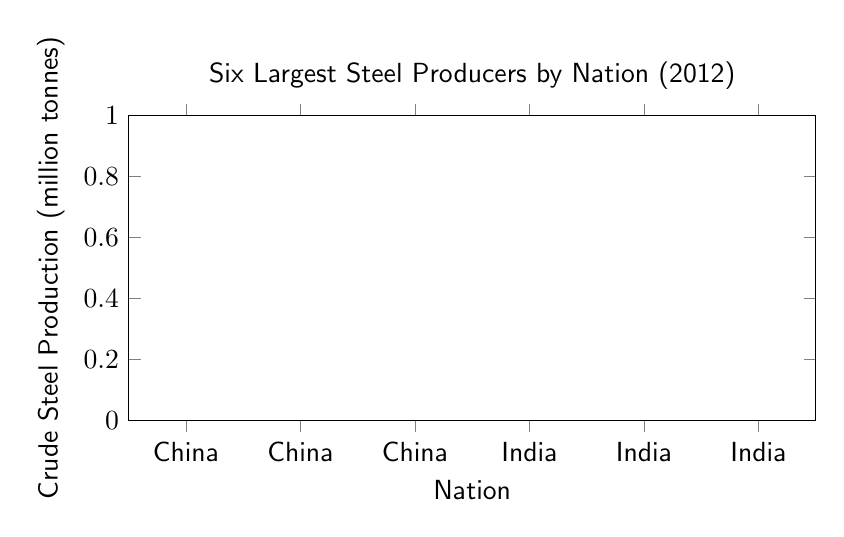
\begin{tikzpicture}
        \begin{axis}[
            ybar,
            bar width=12pt,
            width=0.85\linewidth,
            height=0.45\linewidth,
            xlabel={Nation},
            ylabel={Crude Steel Production (million tonnes)},
            symbolic x coords={China,India,Japan,USA,Russia,South~Korea},
            xtick=data,
            ymin=0,
            ymax=0, % No quantitative data supplied
            nodes near coords,
            every node near coord/.append style={font=\small},
            title={Six Largest Steel Producers by Nation (2012)},
            legend style={at={(0.5,-0.15)},anchor=north,legend columns=-1},
        ]
        % No data provided in source; placeholder empty plot
        \addplot[draw=none] coordinates {};
        \addlegendentry{Data not supplied}
        \end{axis}
    \end{tikzpicture}
    \caption{Bar chart of the six largest steel‑producing nations in 2012 (quantitative values not provided in source).}
\end{figure}

\end{document}